\documentclass{standalone}
\usepackage{tikz}
\usetikzlibrary{patterns, positioning}


\begin{document}
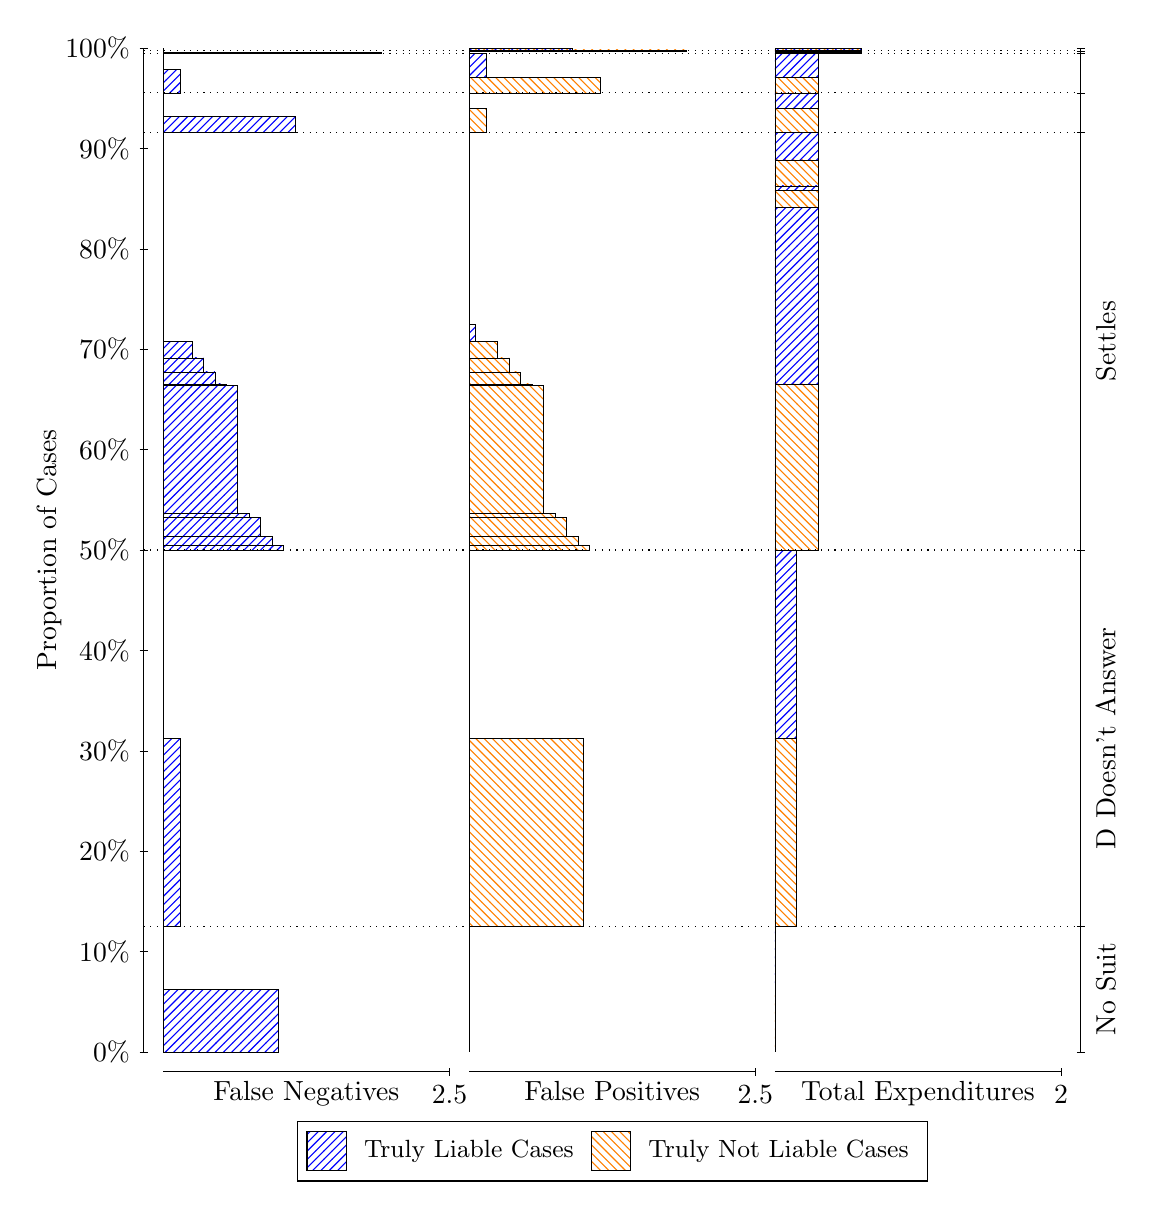
\begin{tikzpicture}
\draw[black, very thin] (1.5,1.75) -- (1.5,14.5);
\node[rotate=90, text=black, anchor=center] at (0.3, 8.125) {Proportion of Cases};
\draw[black, very thin] (1.45,1.75) -- (1.55,1.75);
\node[text=black, anchor=east] at (1.45, 1.75) {0\%};
\draw[black, very thin] (1.45,3.025) -- (1.55,3.025);
\node[text=black, anchor=east] at (1.45, 3.025) {10\%};
\draw[black, very thin] (1.45,4.3) -- (1.55,4.3);
\node[text=black, anchor=east] at (1.45, 4.3) {20\%};
\draw[black, very thin] (1.45,5.575) -- (1.55,5.575);
\node[text=black, anchor=east] at (1.45, 5.575) {30\%};
\draw[black, very thin] (1.45,6.85) -- (1.55,6.85);
\node[text=black, anchor=east] at (1.45, 6.85) {40\%};
\draw[black, very thin] (1.45,8.125) -- (1.55,8.125);
\node[text=black, anchor=east] at (1.45, 8.125) {50\%};
\draw[black, very thin] (1.45,9.4) -- (1.55,9.4);
\node[text=black, anchor=east] at (1.45, 9.4) {60\%};
\draw[black, very thin] (1.45,10.675) -- (1.55,10.675);
\node[text=black, anchor=east] at (1.45, 10.675) {70\%};
\draw[black, very thin] (1.45,11.95) -- (1.55,11.95);
\node[text=black, anchor=east] at (1.45, 11.95) {80\%};
\draw[black, very thin] (1.45,13.225) -- (1.55,13.225);
\node[text=black, anchor=east] at (1.45, 13.225) {90\%};
\draw[black, very thin] (1.45,14.5) -- (1.55,14.5);
\node[text=black, anchor=east] at (1.45, 14.5) {100\%};

\draw[black, very thin] (13.4,1.75) -- (13.4,14.5);
\draw[black, very thin] (13.35,1.75) -- (13.45,1.75);
\node[anchor=west] at (13.35, 1.75) {};
\draw[black, very thin] (13.35,3.3437) -- (13.45,3.3437);
\node[anchor=west] at (13.35, 3.3437) {};
\draw[black, very thin] (13.35,8.125) -- (13.45,8.125);
\node[anchor=west] at (13.35, 8.125) {};
\draw[black, very thin] (13.35,13.432) -- (13.45,13.432);
\node[anchor=west] at (13.35, 13.432) {};
\draw[black, very thin] (13.35,13.93) -- (13.45,13.93);
\node[anchor=west] at (13.35, 13.93) {};
\draw[black, very thin] (13.35,14.428) -- (13.45,14.428);
\node[anchor=west] at (13.35, 14.428) {};
\draw[black, very thin] (13.35,14.464) -- (13.45,14.464);
\node[anchor=west] at (13.35, 14.464) {};
\draw[black, very thin] (13.35,14.5) -- (13.45,14.5);
\node[anchor=west] at (13.35, 14.5) {};

\draw[black, very thin, pattern color=blue, pattern=north east lines] (1.75,1.75) rectangle (3.2033,2.5469);
\draw[black, very thin, pattern color=orange, pattern=north west lines] (1.75,2.5469) rectangle (1.75,3.3438);
\draw[black, very thin, pattern color=blue, pattern=north east lines] (1.75,3.3438) rectangle (1.968,5.7344);
\draw[black, very thin, pattern color=orange, pattern=north west lines] (1.75,5.7344) rectangle (1.75,8.125);
\draw[black, very thin, pattern color=blue, pattern=north east lines] (1.75,8.125) rectangle (3.276,8.1835);
\draw[black, very thin, pattern color=blue, pattern=north east lines] (1.75,8.1835) rectangle (3.1307,8.3019);
\draw[black, very thin, pattern color=blue, pattern=north east lines] (1.75,8.3019) rectangle (2.9853,8.5381);
\draw[black, very thin, pattern color=blue, pattern=north east lines] (1.75,8.5381) rectangle (2.84,8.5931);
\draw[black, very thin, pattern color=blue, pattern=north east lines] (1.75,8.5931) rectangle (2.6947,10.218);
\draw[black, very thin, pattern color=blue, pattern=north east lines] (1.75,10.218) rectangle (2.5493,10.236);
\draw[black, very thin, pattern color=blue, pattern=north east lines] (1.75,10.236) rectangle (2.404,10.387);
\draw[black, very thin, pattern color=blue, pattern=north east lines] (1.75,10.387) rectangle (2.2587,10.565);
\draw[black, very thin, pattern color=blue, pattern=north east lines] (1.75,10.565) rectangle (2.1133,10.779);
\draw[black, very thin, pattern color=orange, pattern=north west lines] (1.75,10.779) rectangle (1.75,13.432);
\draw[black, very thin, pattern color=blue, pattern=north east lines] (1.75,13.432) rectangle (3.4213,13.628);
\draw[black, very thin, pattern color=orange, pattern=north west lines] (1.75,13.628) rectangle (1.75,13.93);
\draw[black, very thin, pattern color=blue, pattern=north east lines] (1.75,13.93) rectangle (1.968,14.232);
\draw[black, very thin, pattern color=orange, pattern=north west lines] (1.75,14.232) rectangle (1.75,14.428);
\draw[black, very thin, pattern color=blue, pattern=north east lines] (1.75,14.428) rectangle (4.5113,14.441);
\draw[black, very thin, pattern color=orange, pattern=north west lines] (1.75,14.441) rectangle (1.75,14.464);
\draw[black, very thin, pattern color=orange, pattern=north west lines] (1.75,14.464) rectangle (1.75,14.477);
\draw[black, very thin, pattern color=blue, pattern=north east lines] (1.75,14.477) rectangle (1.75,14.5);
\draw[black, very thin, pattern color=orange, pattern=north west lines] (5.6333,1.75) rectangle (5.6333,2.5469);
\draw[black, very thin, pattern color=blue, pattern=north east lines] (5.6333,2.5469) rectangle (5.6333,3.3438);
\draw[black, very thin, pattern color=orange, pattern=north west lines] (5.6333,3.3438) rectangle (7.0867,5.7344);
\draw[black, very thin, pattern color=blue, pattern=north east lines] (5.6333,5.7344) rectangle (5.6333,8.125);
\draw[black, very thin, pattern color=orange, pattern=north west lines] (5.6333,8.125) rectangle (7.1593,8.1835);
\draw[black, very thin, pattern color=orange, pattern=north west lines] (5.6333,8.1835) rectangle (7.014,8.3019);
\draw[black, very thin, pattern color=orange, pattern=north west lines] (5.6333,8.3019) rectangle (6.8687,8.5381);
\draw[black, very thin, pattern color=orange, pattern=north west lines] (5.6333,8.5381) rectangle (6.7233,8.593);
\draw[black, very thin, pattern color=orange, pattern=north west lines] (5.6333,8.593) rectangle (6.578,10.218);
\draw[black, very thin, pattern color=orange, pattern=north west lines] (5.6333,10.218) rectangle (6.4327,10.236);
\draw[black, very thin, pattern color=orange, pattern=north west lines] (5.6333,10.236) rectangle (6.2873,10.387);
\draw[black, very thin, pattern color=orange, pattern=north west lines] (5.6333,10.387) rectangle (6.142,10.565);
\draw[black, very thin, pattern color=orange, pattern=north west lines] (5.6333,10.565) rectangle (5.9967,10.779);
\draw[black, very thin, pattern color=blue, pattern=north east lines] (5.6333,10.779) rectangle (5.706,10.992);
\draw[black, very thin, pattern color=blue, pattern=north east lines] (5.6333,10.992) rectangle (5.6333,13.432);
\draw[black, very thin, pattern color=orange, pattern=north west lines] (5.6333,13.432) rectangle (5.8513,13.735);
\draw[black, very thin, pattern color=blue, pattern=north east lines] (5.6333,13.735) rectangle (5.6333,13.93);
\draw[black, very thin, pattern color=orange, pattern=north west lines] (5.6333,13.93) rectangle (7.3047,14.126);
\draw[black, very thin, pattern color=blue, pattern=north east lines] (5.6333,14.126) rectangle (5.8513,14.428);
\draw[black, very thin, pattern color=orange, pattern=north west lines] (5.6333,14.428) rectangle (5.6333,14.45);
\draw[black, very thin, pattern color=blue, pattern=north east lines] (5.6333,14.45) rectangle (5.6333,14.464);
\draw[black, very thin, pattern color=orange, pattern=north west lines] (5.6333,14.464) rectangle (8.3947,14.477);
\draw[black, very thin, pattern color=blue, pattern=north east lines] (5.6333,14.477) rectangle (6.9413,14.5);
\draw[black, very thin, pattern color=orange, pattern=north west lines] (9.5167,1.75) rectangle (9.5167,2.5469);
\draw[black, very thin, pattern color=blue, pattern=north east lines] (9.5167,2.5469) rectangle (9.5167,3.3438);
\draw[black, very thin, pattern color=orange, pattern=north west lines] (9.5167,3.3438) rectangle (9.7892,5.7344);
\draw[black, very thin, pattern color=blue, pattern=north east lines] (9.5167,5.7344) rectangle (9.7892,8.125);
\draw[black, very thin, pattern color=orange, pattern=north west lines] (9.5167,8.125) rectangle (10.062,10.236);
\draw[black, very thin, pattern color=blue, pattern=north east lines] (9.5167,10.236) rectangle (10.062,12.476);
\draw[black, very thin, pattern color=orange, pattern=north west lines] (9.5167,12.476) rectangle (10.062,12.69);
\draw[black, very thin, pattern color=blue, pattern=north east lines] (9.5167,12.69) rectangle (10.062,12.748);
\draw[black, very thin, pattern color=orange, pattern=north west lines] (9.5167,12.748) rectangle (10.062,13.078);
\draw[black, very thin, pattern color=blue, pattern=north east lines] (9.5167,13.078) rectangle (10.062,13.432);
\draw[black, very thin, pattern color=orange, pattern=north west lines] (9.5167,13.432) rectangle (10.062,13.735);
\draw[black, very thin, pattern color=blue, pattern=north east lines] (9.5167,13.735) rectangle (10.062,13.93);
\draw[black, very thin, pattern color=orange, pattern=north west lines] (9.5167,13.93) rectangle (10.062,14.126);
\draw[black, very thin, pattern color=blue, pattern=north east lines] (9.5167,14.126) rectangle (10.062,14.428);
\draw[black, very thin, pattern color=orange, pattern=north west lines] (9.5167,14.428) rectangle (10.607,14.45);
\draw[black, very thin, pattern color=blue, pattern=north east lines] (9.5167,14.45) rectangle (10.607,14.464);
\draw[black, very thin, pattern color=orange, pattern=north west lines] (9.5167,14.464) rectangle (10.607,14.477);
\draw[black, very thin, pattern color=blue, pattern=north east lines] (9.5167,14.477) rectangle (10.607,14.5);
\draw[black, dotted] (1.5,3.3438) -- (13.4,3.3438);
\draw[black, dotted] (1.5,8.125) -- (13.4,8.125);
\draw[black, dotted] (1.5,13.432) -- (13.4,13.432);
\draw[black, dotted] (1.5,13.93) -- (13.4,13.93);
\draw[black, dotted] (1.5,14.428) -- (13.4,14.428);
\draw[black, dotted] (1.5,14.464) -- (13.4,14.464);
\draw[black, very thin] (1.75,1.5) -- (5.3833,1.5);
\node[text=black, anchor=north] at (3.5667, 1.5) {False Negatives};
\draw[black, very thin] (5.3833,1.45) -- (5.3833,1.55);
\node[text=black, anchor=north] at (5.3833, 1.45) {2.5};

\draw[black, very thin] (5.6333,1.5) -- (9.2667,1.5);
\node[text=black, anchor=north] at (7.45, 1.5) {False Positives};
\draw[black, very thin] (9.2667,1.45) -- (9.2667,1.55);
\node[text=black, anchor=north] at (9.2667, 1.45) {2.5};

\draw[black, very thin] (9.5167,1.5) -- (13.15,1.5);
\node[text=black, anchor=north] at (11.333, 1.5) {Total Expenditures};
\draw[black, very thin] (13.15,1.45) -- (13.15,1.55);
\node[text=black, anchor=north] at (13.15, 1.45) {2};

\node[text=black, centered, rotate=90] at (13.72, 2.5469) {No Suit};
\node[text=black, centered, rotate=90] at (13.72, 5.7344) {D Doesn't Answer};
\node[text=black, centered, rotate=90] at (13.72, 10.779) {Settles};





\draw (7.449999999999999,1.5) node[draw=none] (baseCoordinate) {};
\begin{scope}[align=center]
        \matrix[scale=0.5, draw=black, below=0.5cm of baseCoordinate, nodes={draw}, column sep=0.1cm]{
            \node[rectangle, draw, minimum width=0.5cm, minimum height=0.5cm, pattern color=blue, pattern=north east lines] {}; &
            \node[draw=none, font=\small, text=black] (B) {Truly Liable Cases}; &
            \node[rectangle, draw, minimum width=0.5cm, minimum height=0.5cm, pattern color=orange, pattern=north west lines] {}; &
            \node[draw=none, font=\small, text=black] (B) {Truly Not Liable Cases}; \\
            };
\end{scope}

\end{tikzpicture}
\end{document}